\documentclass{standalone}
\usepackage{tikz}
\usetikzlibrary{patterns, positioning}
\usepackage[sfdefault]{ClearSans} %% option 'sfdefault' activates Clear Sans as the default text font
\usepackage[T1]{fontenc}

\begin{document}
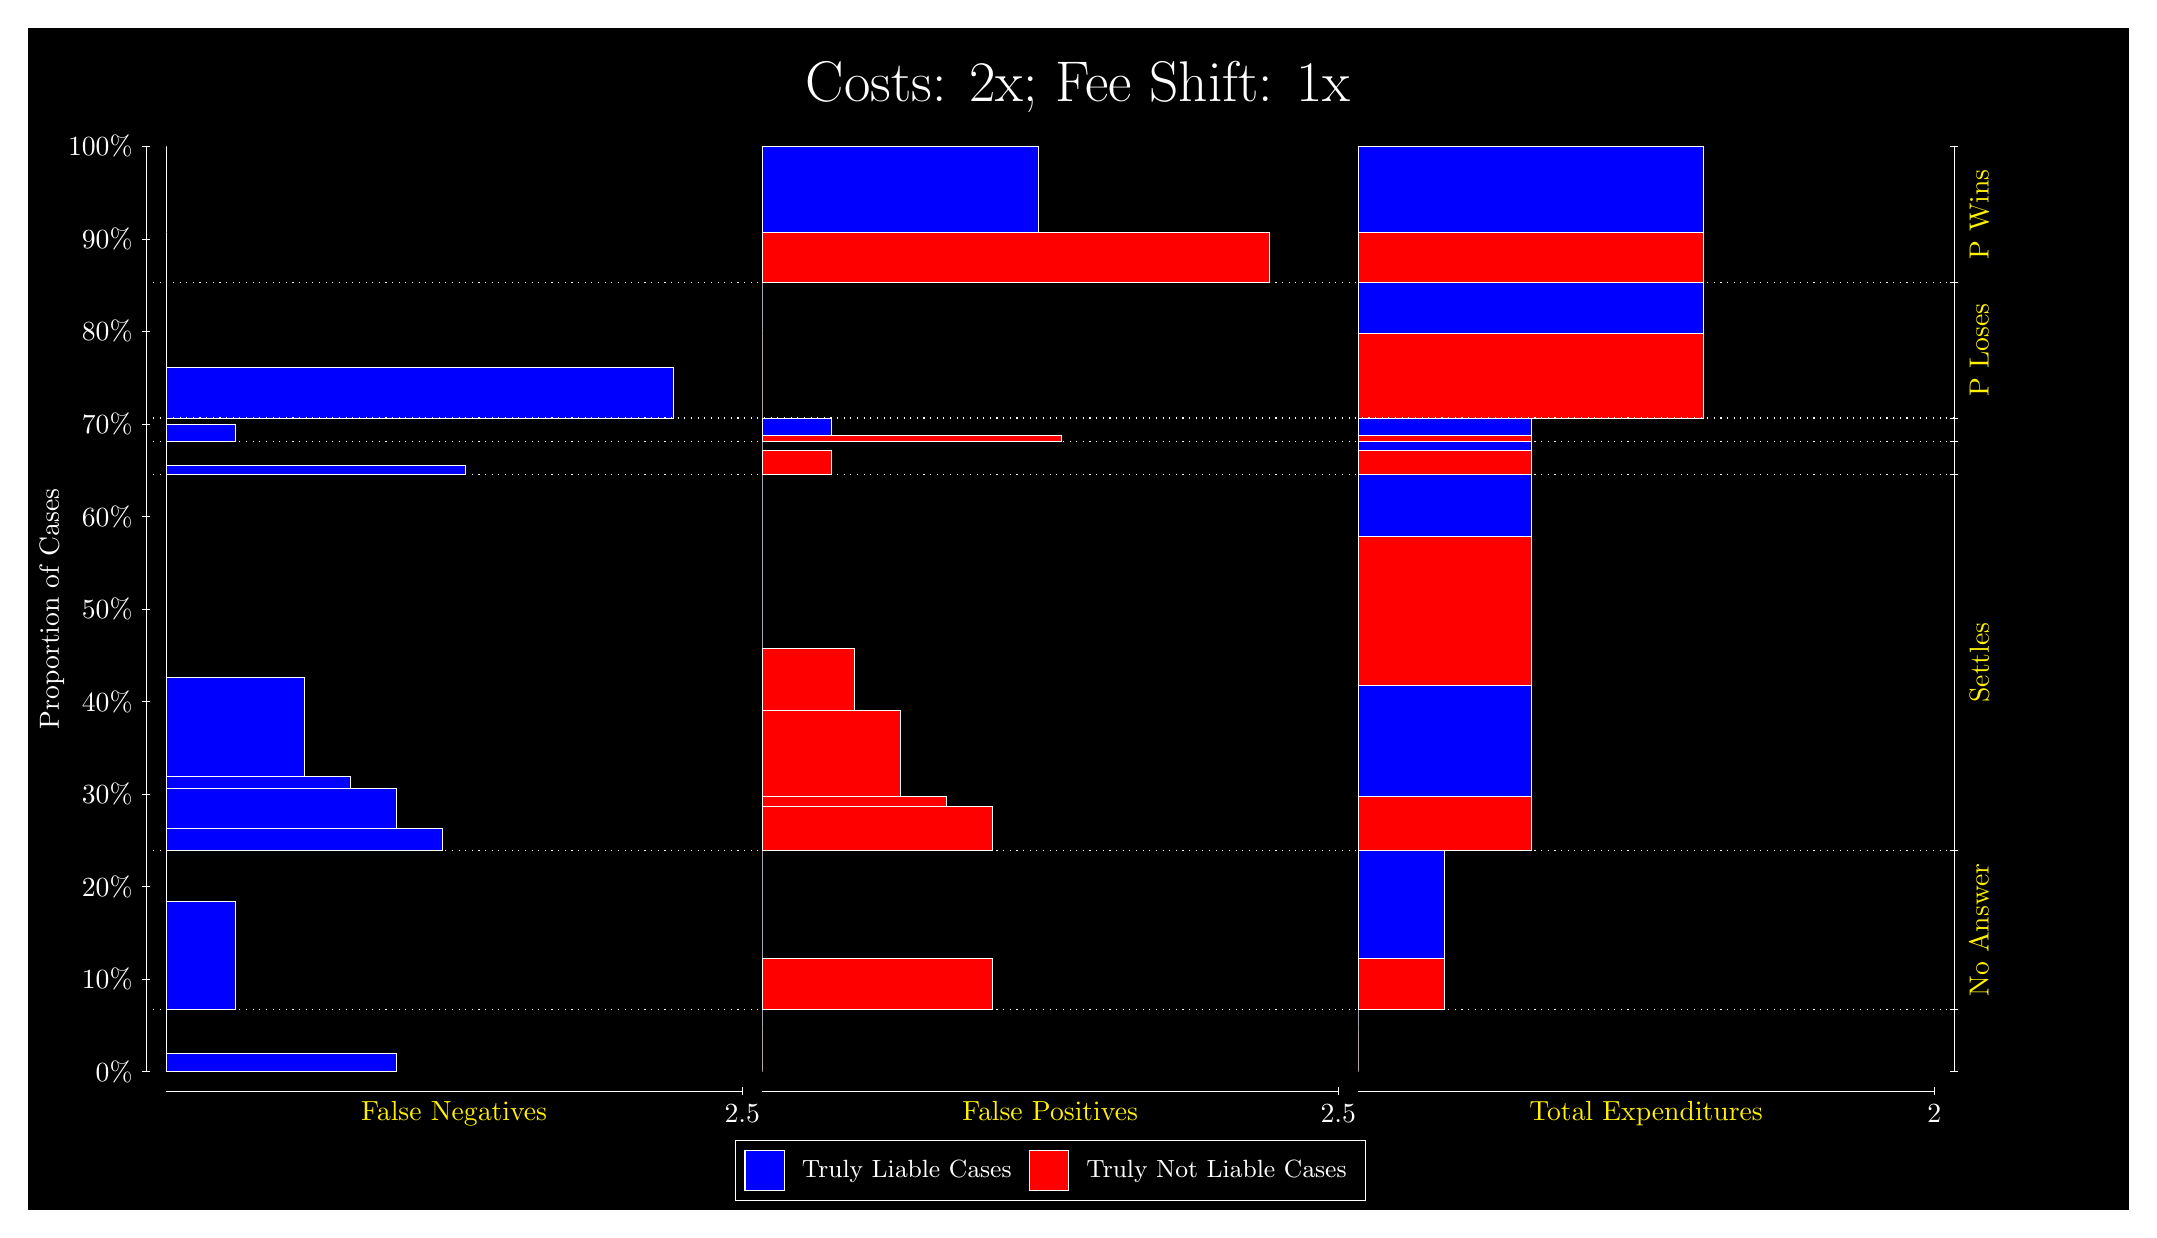
\begin{tikzpicture}
\draw[fill=black] (0,0) rectangle (26.667,15);
\draw[text=white] (0,13.5) rectangle (26.667,15) node[midway] {\huge Costs: 2x; Fee Shift: 1x};
\draw[white, very thin] (1.5,1.75) -- (1.5,13.5);
\node[rotate=90, text=white, anchor=center] at (0.3, 7.625) {Proportion of Cases};
\draw[white, very thin] (1.45,1.75) -- (1.55,1.75);
\node[text=white, anchor=east] at (1.45, 1.75) {0\%};
\draw[white, very thin] (1.45,2.925) -- (1.55,2.925);
\node[text=white, anchor=east] at (1.45, 2.925) {10\%};
\draw[white, very thin] (1.45,4.1) -- (1.55,4.1);
\node[text=white, anchor=east] at (1.45, 4.1) {20\%};
\draw[white, very thin] (1.45,5.275) -- (1.55,5.275);
\node[text=white, anchor=east] at (1.45, 5.275) {30\%};
\draw[white, very thin] (1.45,6.45) -- (1.55,6.45);
\node[text=white, anchor=east] at (1.45, 6.45) {40\%};
\draw[white, very thin] (1.45,7.625) -- (1.55,7.625);
\node[text=white, anchor=east] at (1.45, 7.625) {50\%};
\draw[white, very thin] (1.45,8.8) -- (1.55,8.8);
\node[text=white, anchor=east] at (1.45, 8.8) {60\%};
\draw[white, very thin] (1.45,9.975) -- (1.55,9.975);
\node[text=white, anchor=east] at (1.45, 9.975) {70\%};
\draw[white, very thin] (1.45,11.15) -- (1.55,11.15);
\node[text=white, anchor=east] at (1.45, 11.15) {80\%};
\draw[white, very thin] (1.45,12.325) -- (1.55,12.325);
\node[text=white, anchor=east] at (1.45, 12.325) {90\%};
\draw[white, very thin] (1.45,13.5) -- (1.55,13.5);
\node[text=white, anchor=east] at (1.45, 13.5) {100\%};

\draw[white, very thin] (24.457,1.75) -- (24.457,13.5);
\draw[white, very thin] (24.407,1.75) -- (24.507,1.75);
\node[anchor=west] at (24.407, 1.75) {};
\draw[white, very thin] (24.407,2.5386) -- (24.507,2.5386);
\node[anchor=west] at (24.407, 2.5386) {};
\draw[white, very thin] (24.407,4.5573) -- (24.507,4.5573);
\node[anchor=west] at (24.407, 4.5573) {};
\draw[white, very thin] (24.407,9.3345) -- (24.507,9.3345);
\node[anchor=west] at (24.407, 9.3345) {};
\draw[white, very thin] (24.407,9.751) -- (24.507,9.751);
\node[anchor=west] at (24.407, 9.751) {};
\draw[white, very thin] (24.407,10.05) -- (24.507,10.05);
\node[anchor=west] at (24.407, 10.05) {};
\draw[white, very thin] (24.407,11.769) -- (24.507,11.769);
\node[anchor=west] at (24.407, 11.769) {};
\draw[white, very thin] (24.407,13.5) -- (24.507,13.5);
\node[anchor=west] at (24.407, 13.5) {};

\draw[white, very thin, fill=blue] (1.75,1.75) rectangle (4.6775,1.9772);
\draw[white, very thin, fill=red] (1.75,1.9772) rectangle (1.75,2.5386);
\draw[white, very thin, fill=blue] (1.75,2.5386) rectangle (2.6283,3.9137);
\draw[white, very thin, fill=red] (1.75,3.9137) rectangle (1.75,4.5573);
\draw[white, very thin, fill=blue] (1.75,4.5573) rectangle (5.2631,4.838);
\draw[white, very thin, fill=blue] (1.75,4.838) rectangle (4.6775,5.3466);
\draw[white, very thin, fill=blue] (1.75,5.3466) rectangle (4.092,5.4991);
\draw[white, very thin, fill=blue] (1.75,5.4991) rectangle (3.5065,6.7617);
\draw[white, very thin, fill=red] (1.75,6.7617) rectangle (1.75,9.3345);
\draw[white, very thin, fill=blue] (1.75,9.3345) rectangle (5.5558,9.4507);
\draw[white, very thin, fill=red] (1.75,9.4507) rectangle (1.75,9.751);
\draw[white, very thin, fill=blue] (1.75,9.751) rectangle (2.6283,9.9665);
\draw[white, very thin, fill=red] (1.75,9.9665) rectangle (1.75,10.05);
\draw[white, very thin, fill=blue] (1.75,10.05) rectangle (8.1906,10.693);
\draw[white, very thin, fill=red] (1.75,10.693) rectangle (1.75,11.769);
\draw[white, very thin, fill=red] (1.75,11.769) rectangle (1.75,12.406);
\draw[white, very thin, fill=blue] (1.75,12.406) rectangle (1.75,13.5);
\draw[white, very thin, fill=red] (9.3189,1.75) rectangle (9.3189,2.3114);
\draw[white, very thin, fill=blue] (9.3189,2.3114) rectangle (9.3189,2.5386);
\draw[white, very thin, fill=red] (9.3189,2.5386) rectangle (12.246,3.1822);
\draw[white, very thin, fill=blue] (9.3189,3.1822) rectangle (9.3189,4.5573);
\draw[white, very thin, fill=red] (9.3189,4.5573) rectangle (12.246,5.1244);
\draw[white, very thin, fill=red] (9.3189,5.1244) rectangle (11.661,5.2404);
\draw[white, very thin, fill=red] (9.3189,5.2404) rectangle (11.075,6.334);
\draw[white, very thin, fill=red] (9.3189,6.334) rectangle (10.49,7.1301);
\draw[white, very thin, fill=blue] (9.3189,7.1301) rectangle (9.3189,9.3345);
\draw[white, very thin, fill=red] (9.3189,9.3345) rectangle (10.197,9.6348);
\draw[white, very thin, fill=blue] (9.3189,9.6348) rectangle (9.3189,9.751);
\draw[white, very thin, fill=red] (9.3189,9.751) rectangle (13.125,9.8347);
\draw[white, very thin, fill=blue] (9.3189,9.8347) rectangle (10.197,10.05);
\draw[white, very thin, fill=red] (9.3189,10.05) rectangle (9.3189,11.126);
\draw[white, very thin, fill=blue] (9.3189,11.126) rectangle (9.3189,11.769);
\draw[white, very thin, fill=red] (9.3189,11.769) rectangle (15.759,12.406);
\draw[white, very thin, fill=blue] (9.3189,12.406) rectangle (12.832,13.5);
\draw[white, very thin, fill=red] (16.888,1.75) rectangle (16.888,2.3114);
\draw[white, very thin, fill=blue] (16.888,2.3114) rectangle (16.888,2.5386);
\draw[white, very thin, fill=red] (16.888,2.5386) rectangle (17.986,3.1822);
\draw[white, very thin, fill=blue] (16.888,3.1822) rectangle (17.986,4.5573);
\draw[white, very thin, fill=red] (16.888,4.5573) rectangle (19.083,5.2404);
\draw[white, very thin, fill=blue] (16.888,5.2404) rectangle (19.083,6.6554);
\draw[white, very thin, fill=red] (16.888,6.6554) rectangle (19.083,8.5451);
\draw[white, very thin, fill=blue] (16.888,8.5451) rectangle (19.083,9.3345);
\draw[white, very thin, fill=red] (16.888,9.3345) rectangle (19.083,9.6348);
\draw[white, very thin, fill=blue] (16.888,9.6348) rectangle (19.083,9.751);
\draw[white, very thin, fill=red] (16.888,9.751) rectangle (19.083,9.8347);
\draw[white, very thin, fill=blue] (16.888,9.8347) rectangle (19.083,10.05);
\draw[white, very thin, fill=red] (16.888,10.05) rectangle (21.279,11.126);
\draw[white, very thin, fill=blue] (16.888,11.126) rectangle (21.279,11.769);
\draw[white, very thin, fill=red] (16.888,11.769) rectangle (21.279,12.406);
\draw[white, very thin, fill=blue] (16.888,12.406) rectangle (21.279,13.5);
\draw[white, dotted] (1.5,2.5386) -- (24.457,2.5386);
\draw[white, dotted] (1.5,4.5573) -- (24.457,4.5573);
\draw[white, dotted] (1.5,9.3345) -- (24.457,9.3345);
\draw[white, dotted] (1.5,9.751) -- (24.457,9.751);
\draw[white, dotted] (1.5,10.05) -- (24.457,10.05);
\draw[white, dotted] (1.5,11.769) -- (24.457,11.769);
\draw[white, very thin] (1.75,1.5) -- (9.0689,1.5);
\node[text=yellow, anchor=north] at (5.4094, 1.5) {False Negatives};
\draw[white, very thin] (9.0689,1.45) -- (9.0689,1.55);
\node[text=white, anchor=north] at (9.0689, 1.45) {2.5};

\draw[white, very thin] (9.3189,1.5) -- (16.638,1.5);
\node[text=yellow, anchor=north] at (12.978, 1.5) {False Positives};
\draw[white, very thin] (16.638,1.45) -- (16.638,1.55);
\node[text=white, anchor=north] at (16.638, 1.45) {2.5};

\draw[white, very thin] (16.888,1.5) -- (24.207,1.5);
\node[text=yellow, anchor=north] at (20.547, 1.5) {Total Expenditures};
\draw[white, very thin] (24.207,1.45) -- (24.207,1.55);
\node[text=white, anchor=north] at (24.207, 1.45) {2};


\node[text=yellow, centered, rotate=90] at (24.777, 3.548) {No Answer};
\node[text=yellow, centered, rotate=90] at (24.777, 6.9459) {Settles};


\node[text=yellow, centered, rotate=90] at (24.777, 10.91) {P Loses};
\node[text=yellow, centered, rotate=90] at (24.777, 12.635) {P Wins};

\draw (12.978300999999998,1.5) node[draw=none] (baseCoordinate) {};
\begin{scope}[align=center]
        \matrix[scale=0.5, draw=white, below=0.5cm of baseCoordinate, nodes={draw}, column sep=0.1cm]{
            \node[rectangle, draw, minimum width=0.5cm, minimum height=0.5cm, fill=blue] {}; &
            \node[draw=none, font=\small, text=white] (B) {Truly Liable Cases}; &
            \node[rectangle, draw, minimum width=0.5cm, minimum height=0.5cm, fill=red] {}; &
            \node[draw=none, font=\small, text=white] (B) {Truly Not Liable Cases}; \\
            };
\end{scope}

\end{tikzpicture}
\end{document}